\section{Where the axis comes from}
\label{sec:formation}

\subsection{Template-free extraction}

Base models do not have chat templates, so we extract the axis using a
template-free interview protocol with persona exemplars and an open question
(Appendix~\ref{app:formation}). On Gemma 3 4B-it, this protocol yields an
\emph{interview-instruct axis} that strongly separates the personas and
steers all 10 held-out questions AI-ward (Table~\ref{tab:bridge}). Because
layer-13 cosine is uninformative (Section~\ref{sec:axis}), we validate this
axis by separation and steering rather than cosine (Table~\ref{tab:bridge},
Appendix~\ref{app:formation}).

\subsection{Base and instruction-tuned models}

Applying the template-free protocol to Gemma 3 4B base and Gemma 3 4B-it shows the persona
contrast predates instruction tuning. In the base model, persona separation exceeds the
permutation null at every tested layer (2.6--3.0$\times$, $p=0.005$), and
steering at its own calibrated dose ($\alpha=1.5$) moves 9 of 10 held-out
questions AI-ward, a $+28$-point mean shift; the instruction-tuned model's
own calibrated dose ($\alpha=4$) moves 10 of 10, a $+132$-point shift
(Table~\ref{tab:bridge}). Instruction tuning strengthens the identity and
changes the default model persona rather than creating it. This contrasts
with \citet{ackerman2024inspection}, who find their self-authorship
direction only in an instruction-tuned model, not the base.
Using base-model per-question means, the interview-instruct axis separates both
personas at the readout layers (AUC 1.000), but no shuffled-label floor was measured
for the base axis, so the cosine comparison does not establish alignment
(Table~\ref{tab:bridge}, Appendix~\ref{app:formation}). Across two neutral
raw-text framings, base replies remain human-ward, while
the instruction-tuned model defaults AI-ward without chat-formatting tokens,
arguing against simple template matching (Table~\ref{tab:bridge},
Appendix~\ref{app:formation}). The default is context-sensitive: switching
from one neutral framing to the interview framing shifts base projection from
$-66$ to $-69$, but instruct projection from $+14$ to $-77$
(Table~\ref{tab:bridge}).

\subsection{When the contrast forms}

We track the identity contrast across ten OLMo 2 7B checkpoints spanning
pretraining (1B to 3896B tokens, then base final) and post-training (SFT, direct
preference optimization (DPO), and Instruct) \citep{olmo2}. Like
\citet{bayazit2025crosscoding}, we compare representations across checkpoints; we construct each
checkpoint's own axis using Eq.~\eqref{eq:axis} and the template-free protocol
(Figure~\ref{fig:formation}; Table~\ref{tab:formation} in
Appendix~\ref{app:formation}). We score Cohen's $d$ across layers for each
checkpoint on held-out questions the axis was not created from, so a high
value reflects separation of the two identities rather than overfitting on
the questions that make up the axis (Figure~\ref{fig:formation};
Appendix~\ref{app:formation}). Layer 0 can already separate the two personas
through surface word choice, yielding a large Cohen's $d$ even without evidence of
a deeper self-representation. We therefore measure the formation using the
highest Cohen's $d$ in deep layers (8--30), minus the layer-0 value at the
same checkpoint. This separates the shallow lexical contribution of prose
from a deeper, less lexically driven separation further into the network. At 5B
tokens, this adjusted effect is only $+2.0$ and the model's replies are still
off-task, so we do not treat it as interpretable evidence of the contrast. By
26B tokens, replies are on-task and the effect has risen to $+6.1$, placing
the earliest interpretable formation between 5B and 26B. By 143B tokens, just
3.7\% of stage 1, it reaches $+10.1$; it declines to $+7.8$ by base final,
then recovers to $+10.8$ in the final Instruct model. Alignment with the final
Instruct axis develops later: cosine reaches 0.810 at
base final and 0.978 at SFT, showing that SFT accounts for most post-training
rotation (Table~\ref{tab:formation}). Raw separation and early cosines give
misleading formation timings (Appendix~\ref{app:formation}), so formation and
convergence are distinct events.

Effective steering is a separate question. Across the three tested
checkpoints, AI-ward steering on each checkpoint's own axis moves held-out
replies (Section~\ref{sec:axis}) by an average of $+17$ points compared to
baseline (Table~\ref{tab:formation}). Human-ward steering remains near chance
(ordering 6 of 10 held-out questions on average), because the unsteered checkpoints
sit deeply human-ward, averaging $-73$ points and leaving little room for further
human-ward movement (Appendix~\ref{app:formation}). As a specificity check on the
Instruct checkpoint, a same-norm random direction remains coherent but orders only 6 of 10
questions AI-ward, versus 8 of 10 for the axis, and moves the mean by just $+4$ points
(Table~\ref{tab:formation}, Appendix~\ref{app:formation}). The human-AI contrast is
behaviorally steerable before its direction converges to the final
instruction-tuned axis. Each checkpoint has its own OLMo-specific axis, so
this tracks the emergence of a human-versus-AI contrast within OLMo rather
than convergence to the Gemma direction.

\begin{figure}[t]
  \centering
  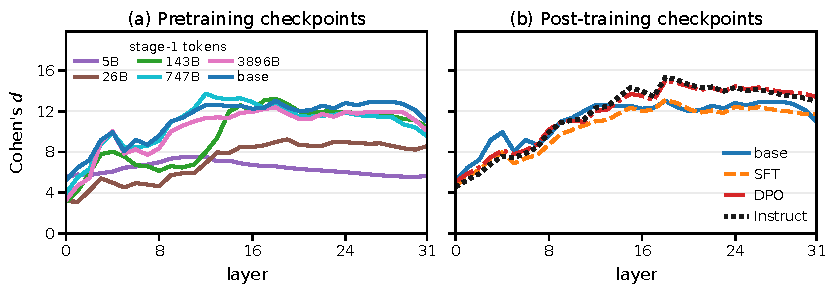
\includegraphics[width=0.95\linewidth]{artifacts/human-AI/formation/formation_heldout.pdf}
  \caption{Layerwise Cohen's $d$ across OLMo 2 7B (a) pretraining and (b)
  post-training checkpoints. The incoherent 1B checkpoint is excluded
  (Table~\ref{tab:formation}).}
  \label{fig:formation}
\end{figure}

\FloatBarrier
